\documentclass[conference]{IEEEtran}
\IEEEoverridecommandlockouts
% The preceding line is only needed to identify funding in the first footnote. If that is unneeded, please comment it out.
\usepackage{cite}
\usepackage{amsmath,amssymb,amsfonts,dsfont}
\usepackage{algorithmic}
\usepackage{graphicx}
\graphicspath{ {images/} }
\usepackage{listings}
\usepackage{textcomp}
\usepackage{xcolor}
\usepackage{xr}
\def\BibTeX{{\rm B\kern-.05em{\sc i\kern-.025em b}\kern-.08em
    T\kern-.1667em\lower.7ex\hbox{E}\kern-.125emX}}

\usepackage{stackengine}
\newcommand\citeequation[2]{%
  \stackengine{0pt}{$\displaystyle#1$}{\makebox[\linewidth]{\hfill \cite{#2}\kern20pt}}
    {O}{c}{F}{T}{L}
}
\begin{document}

\title{Sharing and Binding for General Circuits\\
{\footnotesize }
\thanks{University of Applied Sciences Hamm-Lippstadt.}
}

\author{\IEEEauthorblockN{ Sheikh Muhammad Adib Bin Sh Abu Bakar}
\IEEEauthorblockA{\textit{University of Applied Sciences Hamm-Lippstadt} \\
\textit{B.Eng. Electronic Engineering}\\
Lippstadt, Germany \\
sheikh-muhammad-adib.bin-sh-abu-bakar@stud.hshl.de}

}

\maketitle

\begin{abstract}

Producing an optimum circuit is the dream of every circuit designer. A circuit can be evaluated through its used area and performance. Those aspects are designer concern to be optimized that can be done only during architectural synthesis or known as high level synthesis. Resource sharing and binding are very important process in circuit optimization. In this paper, sharing and binding will be discussed mainly for general circuit. This includes a sample model circuit to ease the explanation process and the method used for sharing and binding. After that, the strategies for optimization that use all those methods will be explored.

\end{abstract}

\begin{IEEEkeywords}
sharing, binding, general circuit, optimization
\end{IEEEkeywords}

\input{Introduction.tex} 
% motivation
% intro to digital circuit synthesis
% intro HLS
% the need of sharing and binding
% general circuit
% output
% analysis of output : are, latency, cycle time -> optimize
% paper flow

\section{Sample Model}
% sample model: integration equation

To make every explanation in upcoming sections easy to understand,  a sample model of a circuit at the architectural level will be used. The model that has been chosen is circuit that solve the following equation :

\begin{equation}
    \citeequation{y\prime\prime + 3xy\prime +3y}{main}\label{diffeq}
\end{equation}

\begin{figure}[ht]
    \centering
    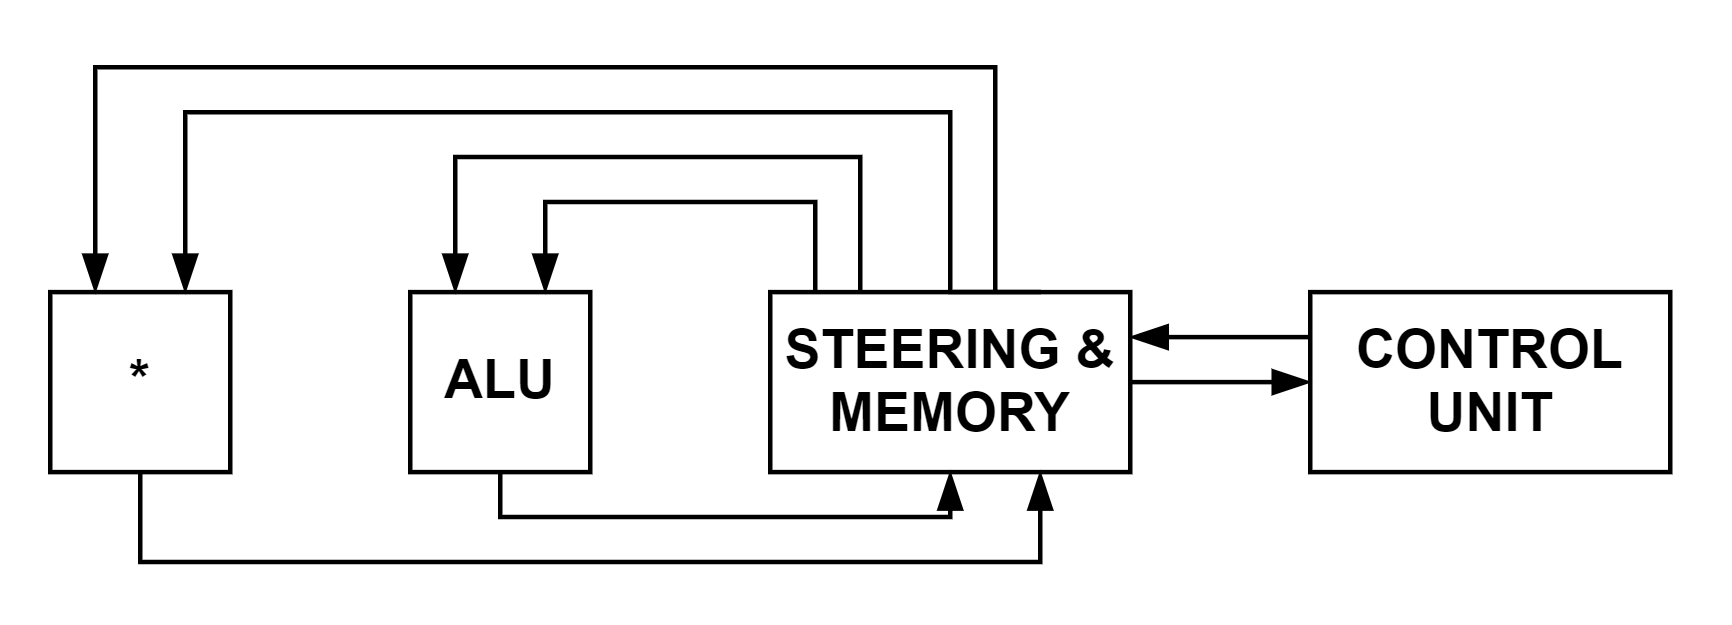
\includegraphics[width=0.35\textwidth]{Example_of_structural_view_at_the_architectural_level}
    \caption{Example of structural view at the architectural level. \cite{main}}
    \label{Example_of_structural_view_at_the_architectural_level}
\end{figure}

The structural view of the model at architectural level is shown in ``Fig. \ref{Example_of_structural_view_at_the_architectural_level}" and the behavioural view of the model at architectural level can be written in HDL as follows \cite{main}:

\begin{lstlisting}
diffeq {
    read(x, y, u, dx, a);
    repeat {
        xl = x + dx ;
        ul = u - ( 3*x*u*dx ) - ( 3*y*dx );
        yl = y + u*dx;
        c = xl < a;
        x = xl ; u = ul ; y = yl;
        }
    intil ( c );
    write ( y );
}
\end{lstlisting}

From the behaviour model, we could see that the solution involving iteration of set of operations. The set of operation in each iteration (within the repeat function) can be broke into 11 simple operation and can be modelled using data-flow graph as shown in ``Fig. \ref{Example_of_a_data-flow_graph}" to represent the abstract model of the solution at architectural level in terms of tasks and their dependencies \cite{main}. The task could be \textit{No-Operation} (NOPs) if the task does not involve any operation or task that can be executed instantaneously without side effect. 

\begin{figure}[ht]
    \centering
    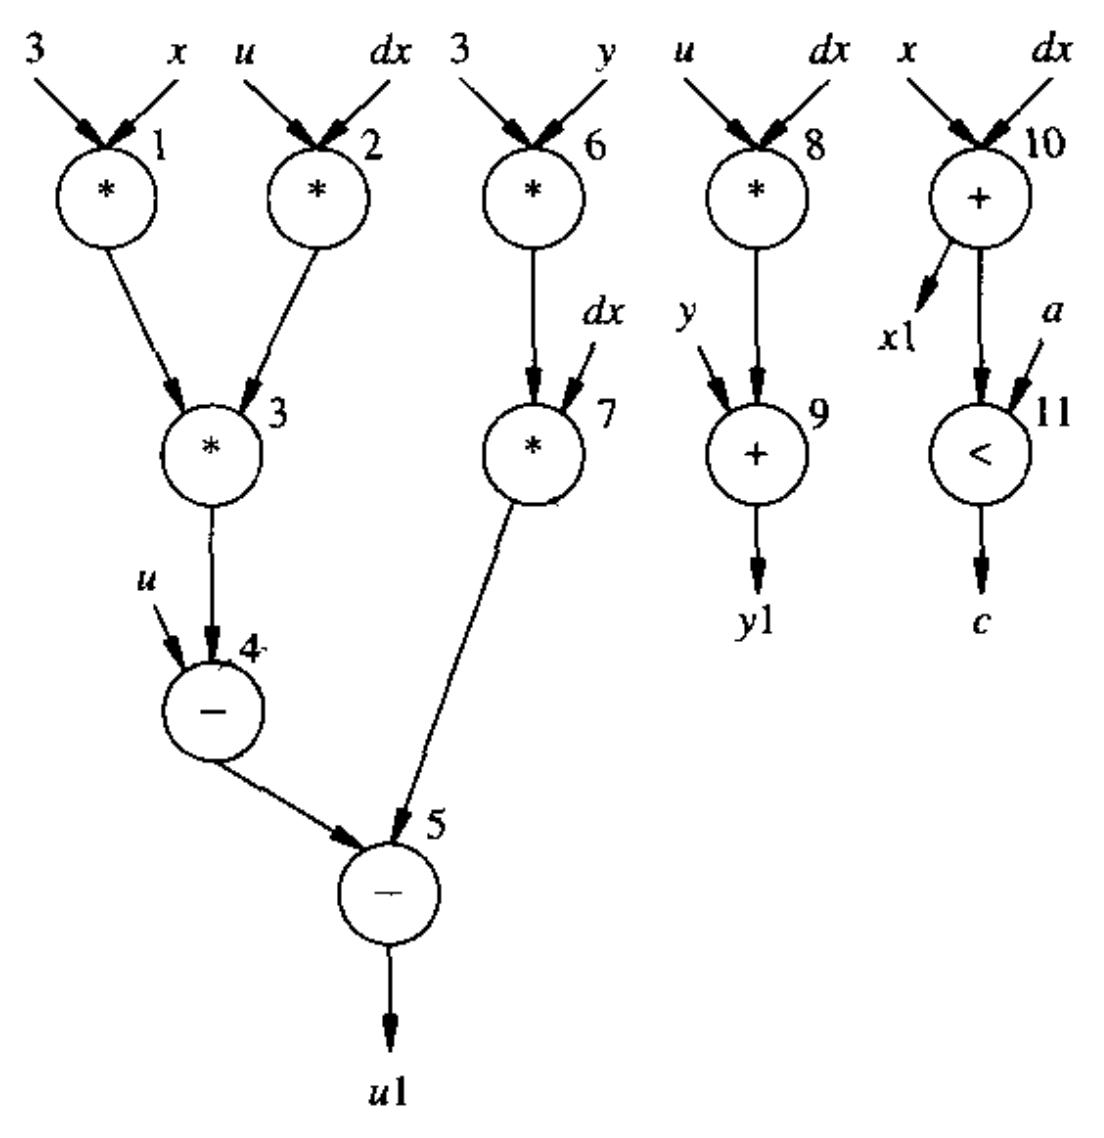
\includegraphics[width=0.35\textwidth]{Example_of_a_data-flow_graph}
    \caption{Example of a data-flow graph. \cite{main}}
    \label{Example_of_a_data-flow_graph}
\end{figure}

Regrading the branching and iteration, the control-flow information can be modelled using a control-flow graph. According to \cite{main}---``Many models have been proposed to represent control data-flow graphs (CDFGs)". One of the main CDFG that will be intensively used in this paper is sequencing graph,  $G_{s}(V, E)$, as illustrate in``Fig. \ref{Example_of_ a_sequencing_graph}" that represent the circuit model where $V$ is the vertex set, $ V = \{v_{i}; i = 0, 1.. . . , n\}$ and $E$ is the set of edges, $ E = \{(v_{i}, v_{j}); i, j = 0, 1, ... , n\} $. 
Based on the ``Fig. \ref{Example_of_ a_sequencing_graph}", the graph has two properties :

\begin{itemize}
    \item Polar : The source and sink vertices are labelled with $v_{0}$ and $v_{n}$ representing the start and the last task.Both are NOPs.
    \item Acyclic : No iteration or loop because the iteration and branching are modelled outside the graph.
\end{itemize}

\begin{figure}[ht]
    \centering
    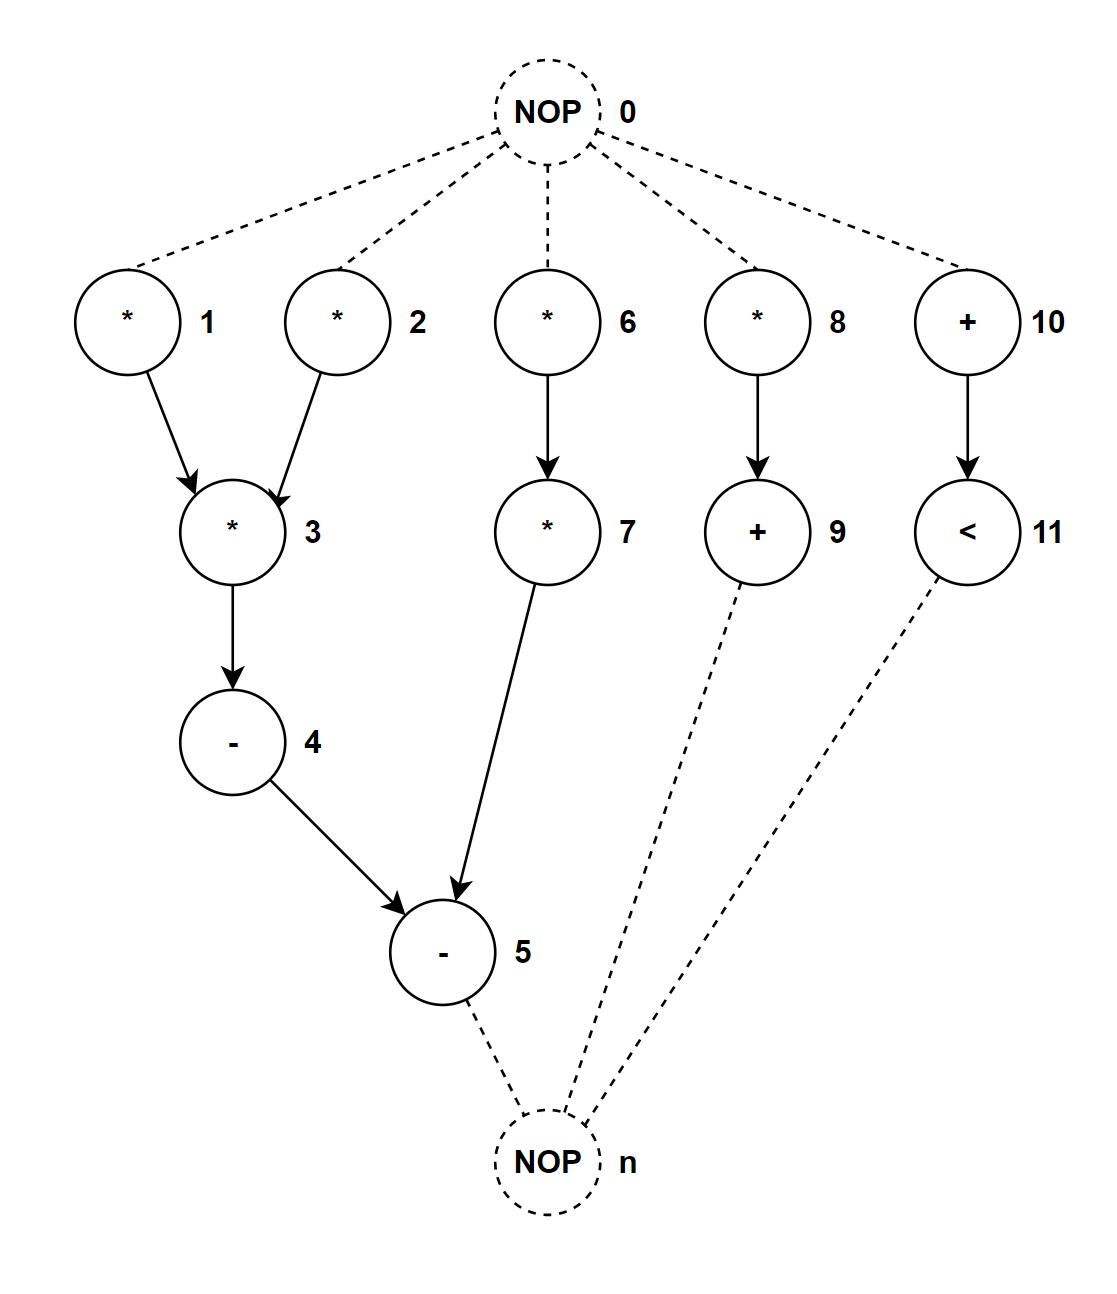
\includegraphics[width=0.35\textwidth]{Example_of_ a_sequencing_graph}
    \caption{Example of a sequencing graph. \cite{main}}
    \label{Example_of_ a_sequencing_graph}
\end{figure}



As stated, the iteration and branching are modelled outside this graph means that path in the graph not representing alternative but concurrent streams of operation \cite{main}. But it does not mean that the sequencing graph cannot model loop and branching. They do, but in a hierarchical way.


After a solution or the circuit have been model, the specification should be further described. The model specification will be explained more in the next sub topic.
% sample model: integration equation

\section{Specification}
% circuit specification
% resource 
% constarint
% sample model : sequence graph
% scheduled equence graph

In pervious section, one of the important specification already be represented in sequencing graph which is the behavioural-level of the circuit model. In this section, the specification will be furthered detailed, including the type and number of resource that will be used in the circuit and the constraints.

At architectural level, resource have their own definition, where it implements different types of function in hardware and can be classified into 3 classes as listed below \cite{main}:

\begin{itemize}
    \item Functional resources : Implementing the arithmetic or logic functions. 
    \item Memory resources : Memory array
    \item Interface resources  : Used to support data transfer including busses and interfacing circuit including external interface for input output
\end{itemize}

Within the scope of this paper, only functional resource will be intensively used. The last specification aspect that will be considered in this paper is constraint. It can be classified into two categories, which are \cite{main}:

\begin{itemize}
    \item Interface constraint : This specification used to ensure that the circuit can be implemented in provided environment like format and timing used in I/O interface.
    \item Implementation constraint : This constraint specified the area constraint, performance constraint and binding constraint.
\end{itemize}

All the constraint are must not specify to give some freedom in synthesizing the architectural model. To narrow the scope of this paper,  the performance constraint will be used including cycle time and latency bound, $\lambda$ that are used to extend the pervious sequencing graph to scheduled sequencing graph as illustrate in ``Fig. \ref{scheduled_sequencing_graph}". Scheduled graph is a function $\varphi : V \xrightarrow{} Z^{+}$, where $\varphi(v_{i})$, denotes the operation start time such that $t_{i} \leq t|_{j} + d_{j}, \forall{i,j}:(v_{j},v_{i}) \in E$ \cite{main}. This graph will be used for further synthesis process.The area constraint entail the number of resource usage, since adding more resource means adding more area to the circuit. All constraint will be further explained in upcoming sections.
 
\begin{figure}[ht]
    \centering
    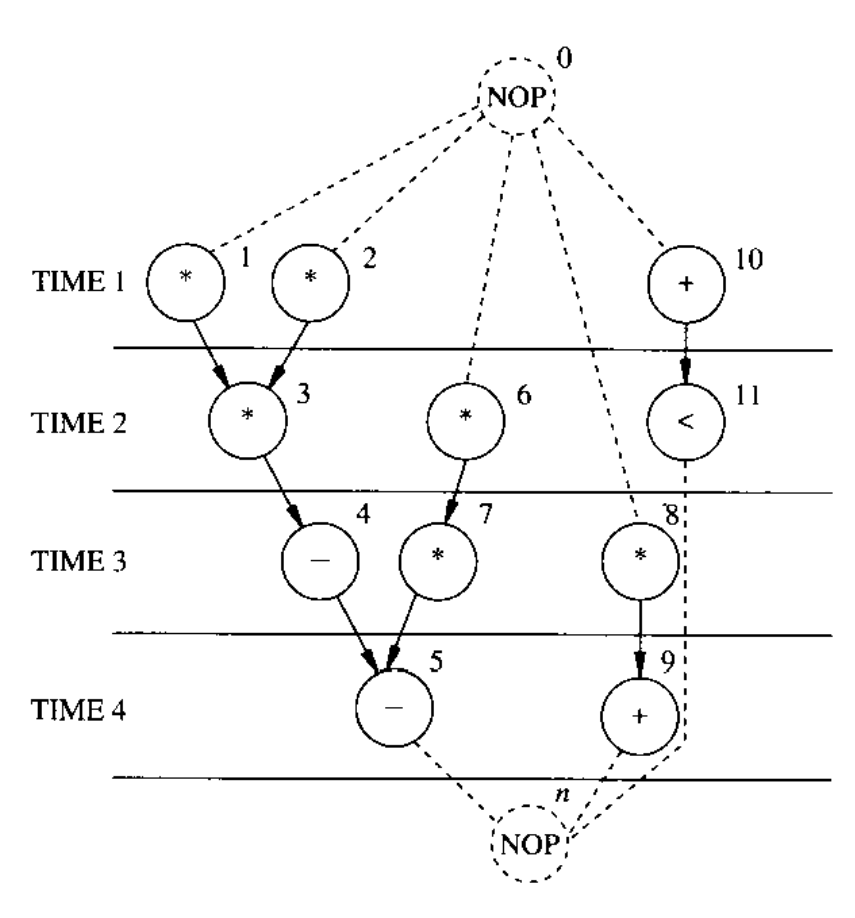
\includegraphics[width=0.5\textwidth]{scheduled_sequencing_graph}
    \caption{scheduled sequencing graph. \cite{main}}
    \label{scheduled_sequencing_graph}
\end{figure}

As shown in `Fig. \ref{scheduled_sequencing_graph}", each vertex represent a type of computation or known as operation type and the resource that execute the operation called resource type. It is also possible that a resource type could execute more than one operation type. ALU, for instance, can do addition, subtraction and comparison. In our circuit model, the resource type that we used is ALU and multiplier as shown in ``Fig. \ref{Example_of_structural_view_at_the_architectural_level}". 

Before going further to the synthesizing process, the stage of the synthesizing process need to be understood. The stages will be discussed in the next section. 
% circuit specification
% resource 
% constarint
% sample model : sequence graph
% scheduled equence graph

\section{Architectural Synthesis Stages}
% stages : placing and interconnection
% focus more on interconnection 
In architectural level synthesis, two stages are involved \cite{main}, which are :

\begin{itemize}
    \item Placing the operation in time and space.
    \item Determining the detailed interconnection of the data path and the logic level specification of the control unit.
\end{itemize}

To narrow down the scope of this paper, only the first stages will be discussed. In the next section, the important process in the first stage will be explained. 
% stages : placing and interconnection
% focus more on interconnection 



\section{Resource Sharing And Binding Methods}

% sharing def
% binding def
% problem - The Spatial Domain: Binding 

% sharing and binding method 

% Non-Hierarchical Sequencing Graphs 
% Hierarchical Sequencing Graphs 

% Register Sharing 
% Multi-Port Memory Binding 
% Bus Sharing and Binding 
% UnconsIrGned Minimum-Area Binding* 
% Performance-ConsIrained and Performance-Directed Binding*

In this section one of the most important processes in synthesizing an architecture model will be discussed which is resource sharing and binding. We assume here scheduled sequencing graph and non-hierarchical sequencing graph only. Before going through the methods used to solve resource sharing and binding problem, the definition of them should be comprehended as follows \cite{main}:

\begin{itemize}
    \item Resource sharing : A resource is assigned to more than one operation
    \item Binding : Mapping of an operation to a physical resource, $\beta : V \xrightarrow{} R * Z^{+}$, where $\beta(v_{i})$, where $\beta(v_{i})=(t,r)$ denotes that the operation corresponding to $v_{i} \in V$, with type $\tau(c_{i}) = t$, is implemented by the $r^{th}$ instance of resource type $t \in R$ for each $i = 1,2,...,n_{ops}$
\end{itemize}

If more than one operation with the same type are used, like in our sample model, resource sharing can be implemented as long as the operations are not concurrent, means that $ E=\{(v_{i},v_{j})|\tau(v_{i}=v_{j} $ and $ ((t_{i}=d_{i} \leq t_{j}) $ or $ t_{j}=d{j} \leq t_{i})),i,j=1,...,n_{ops}\}$. The operation is \textit{compatible} if those conditions are met \cite{main}. The need of sharing is to reduce the area of a circuit. Some circuit specification already have area constraint that need to be followed, means that resource sharing need to be applied. It is also possible that the binding constraint already specified in a circuit specification. To reduce the complexity, our model circuit does not have binding constraint, but area constraint maybe applied and will be explained later. Many methods have been proposed to help designer to decide which operations are compatible and how many resources should be used. Resource sharing implicitly describe the binding of an operation to a specific resource. That means every method used to solve resource sharing problem involve binding problem. 

Next, we will discuss the methods used to determine the compatibility of operation for sharing. First, for the sake of simplicity, we assume that our model circuit is a resource dominated circuit, and then we will assume our model circuit is a general circuit to help the reader understand the method. 

\subsection{Compatibility Graph}

 One of the method to analyse the compatibility of operation for sharing is using Compatibility graph. Compatibility graph, $G_{+}(V,E)$ is a graph whose vertex set  $  V = \{v_{i}, i = 1,2,..., n_{ops}\} $ is in one to one correspondence with the operation and whose edge set $ E = \{\{v_{i},v_{j} i,j = 1,2,...,n_{ops}\}$ denotes the compatible operation pairs \cite{main}. This means that the number of distinct components in the graph is at least equal to the number of resource categories. An optimal resource sharing strategy is one that reduces the amount of resources instance required\cite{main}.
 
 According to \cite{main}---``A group of mutually compatible operations corresponds to a subset of vertices that are all mutually connected by edges, i.e., to a clique. Therefore, a minimal set of mutually compatible operations is represented by a maximal clique in the compatibility graph. Since we can associate a resource instance to each clique, the problem is equivalent to partitioning the graph into a minimum number of cliques. Such a number is the clique cover number of $G_{+}(V,E)  $, denoted by $\kappa(G_{+}(V,E)) $"

 Base on our sample model, the compatibility graph can be drawn as in ``Fig. \ref{Compatibility_graph}. Each vertex representing the operation type. We can see that $\{v_{2},v_{6}\} $ and $\{v_{10},v_{11}\} $ are examples of compatible operation.  Examples of cliques are the sub-graphs induced by $\{v_{1},v_{3},v_{7}\}  $,$\{ v_{2},v_{6},v_{8}\} $,$\{ v_{4},v_{5}, v_{10}, v_{11}\}$ $ \{v_{9}\} $. So the clique cover number $ \kappa $ of the graph is 4, corresponding to two multipliers and two ALUs. The edges of a clique are thicker than the other, as shown in ``Fig. \ref{Compatibility_graph}.
 

\begin{figure}[h]
    \centering
    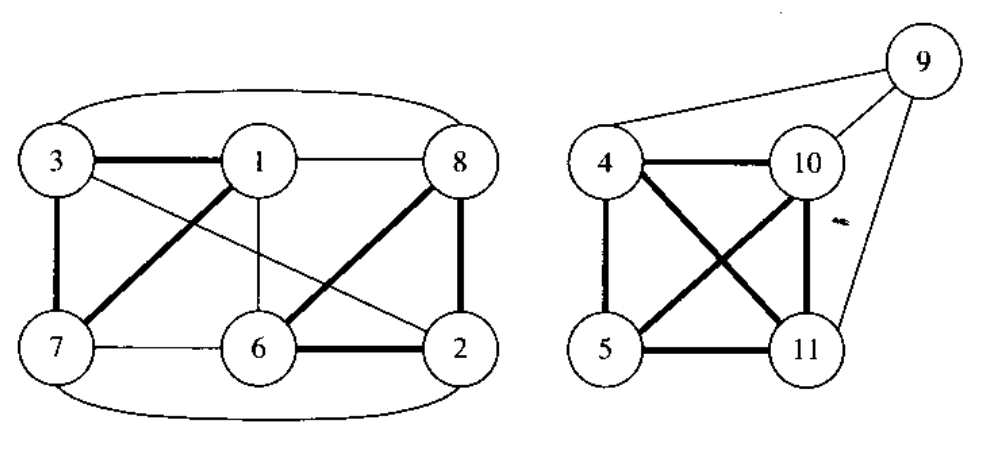
\includegraphics[width=0.4\textwidth]{Compatibility_graph}
    \caption{ Compatibility graph. \cite{main}}
    \label{Compatibility_graph}
\end{figure}

Since the area of a general circuit is not only depends on resource but also involving the area of steering logic and wiring, we need to extend the compatibility graph to help designer estimate area more accurately. To make explanation much simpler, we only focus on the multiplexer, whose  area and propagation delays depend on the number of inputs and wires \cite{main}.

We extend the compatibility graph to a weighted compatibility graph.  Different types of weighted compatibility graphs can be defined \cite{main}. As mentioned before, we can represent the sub-graph as a clique. Cliques may be connected with weight. The cost of allocating the clique to a single resource comprehend the cost of steering logic and wiring components like multiplexers.

A set inclusion cost function can be used to create a weighted compatibility graph model \cite{main}. Each vertex of the compatibility graph in this model is assigned a set of weights known as a cost set. The total cost is the sum of all weights associated with a partition's cliques. The cost-set approach allows us to compute weights on cliques based on vertices' properties. This model may be used to describe the steering logic and wiring area, which are dependent on operation grouping and binding to a shared resource.

Now we consider the operation in ``Fig. \ref{Compatibility_graph}" within the first clique that use multiplier. Assuming that the cost of multiplexing $a$ signal is $area_{mux} = area_{mux}^{ \bigtriangleup}(a-1)$ and is expressed as $area_{M}^{0} = \sum_{i=1}^{a} area_{M}^{i}$, where $area_{mux}^{ \bigtriangleup}=area_{M}^{i}= -area_{M}^{0}$, $1 \leq i \leq a$ \cite{main}.

If we assume each operation with dedicated resource, the overall cost is $(area_{*} + area_{M}^{0}) + \sum_{i=1}^{3} area_{M}^{i}  = 3area_{*}$. If we assume operation $v_{3}$ and $v_{1}$ share the same resource, and $v_{7}$ with dedicated resource, the overall cost is $(area_{*} + area_{M}^{0} +\sum_{i=1}^{3} area_{M}^{i}) + (area_{*},area_{M}^{0},area_{M}^{3})  = 2area_{*} + area_{mux}^{ \bigtriangleup}(2-1)$.

So, we can conclude that this method  could help designer to decide the compatibility of operations under the constrained area. Another technique that based on compatible graph as mention in \cite{main} that purposed by Tseng and Siewiorek is clique partitioning algorithm that constructs cliques from compatible pairs of operations. Means that they utilized edge weights to reflect the intensity of desire for sharing. The edge-weighted compatibility graph is denoted here by $G_{+}(V, E, W)$.

Again, we consider the operation in ``Fig. \ref{Compatibility_graph}". The subgraph's two vertices with the most common neighbours are merged. If the edge is not connected to all the member of the new vertex (clique seed), the edge will be deleted. This process is repeated until no connected edge left. Then the formed clique will be saved on a list.  This process can be illustrated in ``Fig. \ref{Comparibility_graph_mux_2}"

\begin{figure}[h]
    \centering
    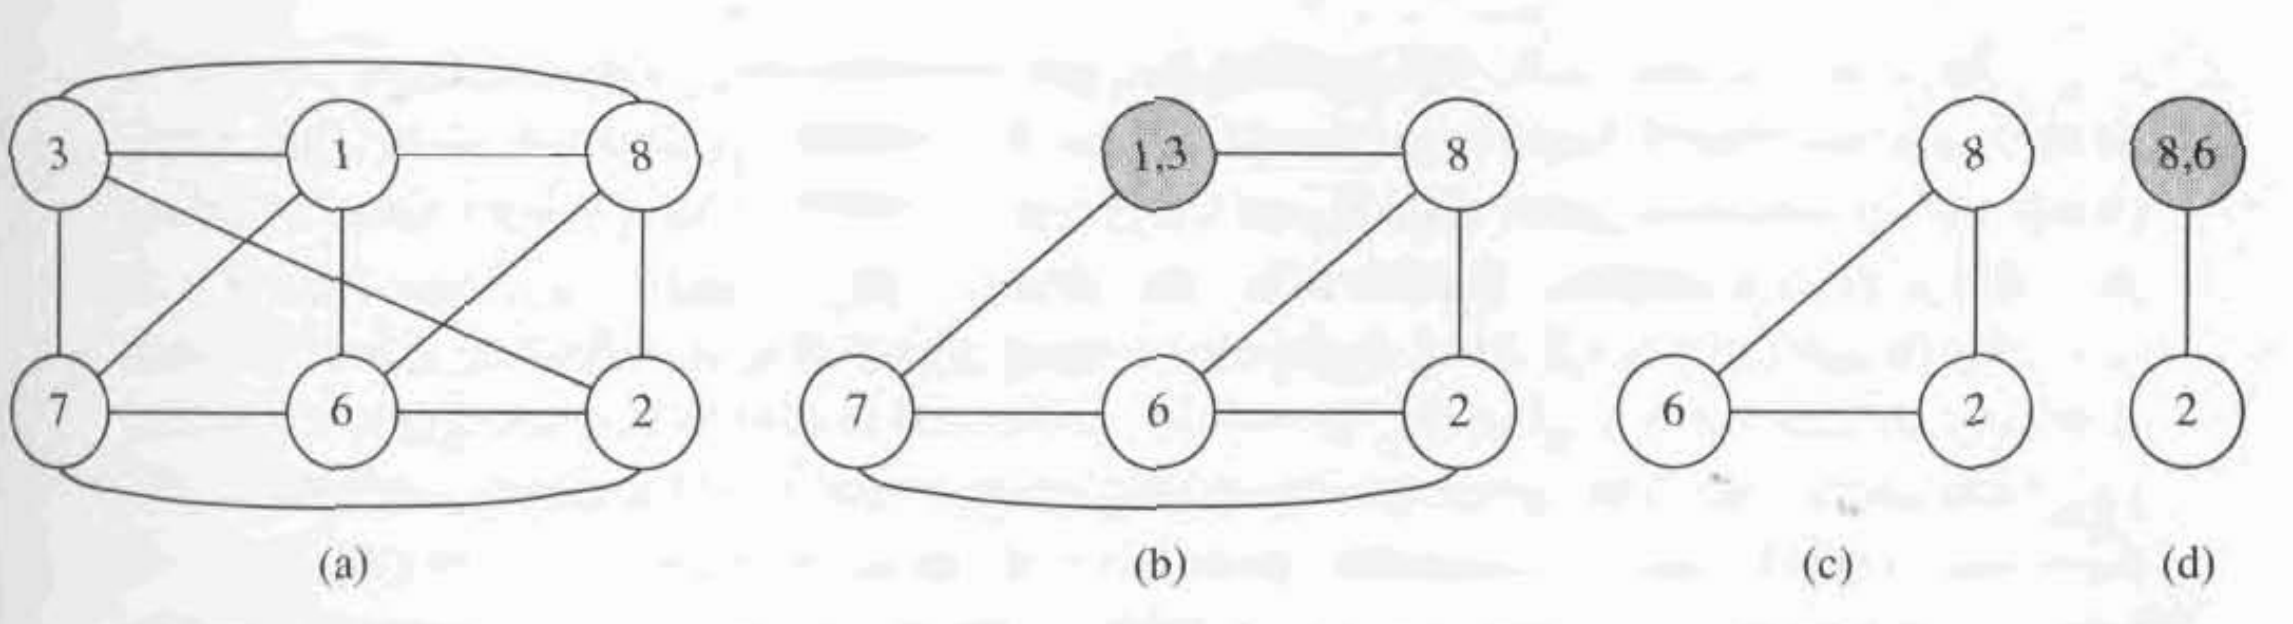
\includegraphics[width=0.5\textwidth]{Comparibility_graph_mux_2}
    \caption{ (a) Compatibility graph for the multiplier type. (b) Reduced compatibility graph with clique seed. (c) Fragment of compatibility graph after one clique has been removed. (d) Reduced fragment with clique seed. \cite{main}}
    \label{Comparibility_graph_mux_2}
\end{figure}

Next, we will go through  another method used to analyse the compatibility of operation for sharing other than compatibility graph, which is conflict graph.


\subsection{Conflict Graph}

Compatibility of operation for sharing can be analysed using Conflict graph. Conflict graph, $G_{-}(V, E)$ is a graph, is a graph whose vertex set $ V = \{ v_{i}, i = 1, 2, ..., n_{ops}\}$ is in one-to-one correspondence with the operations and whose edge set $E = \{\{v_{i},v_{j}\} i, j = 1, 2, ...,n_{ops}\}$ denotes the conflicting operation pairs.Operations have conflict when they are not compatible \cite{main}. Means that the graph is the compliment of the compatibility graph because a subset of vertices that are not linked by edges corresponds to a set of mutually compatible operations.

The vertexes of the graph are coloured accordingly based on their compatibility, so that it will help the designer to solve the sharing problem. Each colour represent different resource, and it will be helpful if operation with different resource type are distinguished first because they are obviously always conflicting. The optimum resource sharing is when minium number of colour used, which are denoted by $\chi(G_{-}(V, E))$.  $\chi(G_{-}(V, E))$ is equal to $\kappa(G_{+}(V, E))$.

Again, using our sample model, the coloured conflict graph can be drawn as illustrate in ``Fig. \ref{Conflict_graphs_for_the_mtlltiplier_and_ALU_types}.


\begin{figure}[h]
    \centering
    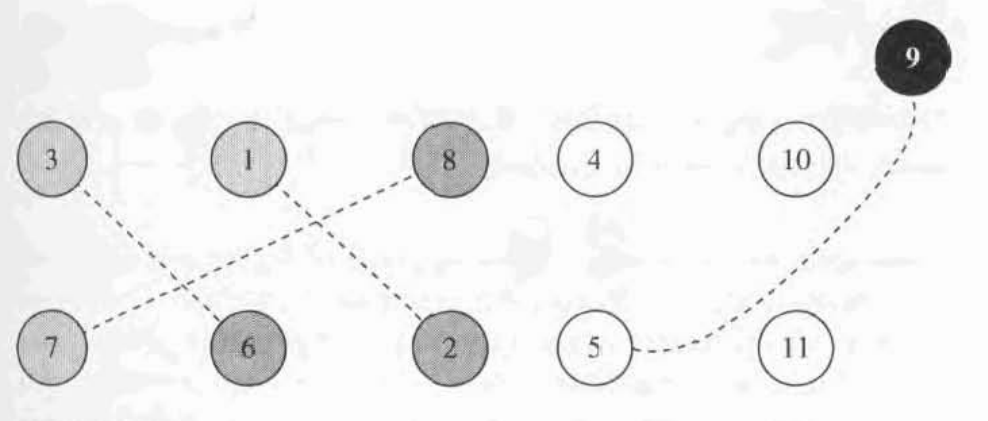
\includegraphics[width=0.4\textwidth]{Conflict_graphs_for_the_mtlltiplier_and_ALU_types}
    \caption{Conflict graphs for the multiplier and ALU types. \cite{main}}
    \label{Conflict_graphs_for_the_mtlltiplier_and_ALU_types}
\end{figure}

The execution delay for each operation is $\{[t_{i}, t_{i} + d_{i} - 1 ]; i + 1, 2, ...,n_{ops}$ and the edges of the conflict graph denote intersections among intervals, hence they are in an interval graph \cite{main}. Means that, in polynomial time, by applying interval sequence graph, it is much easier for designer to find the minimum number of colour used. Back to our circuit model in ``Fig. \ref{scheduled_sequencing_graph}", interval conflict graph can be obtained as shown in ``Fig. \ref{Intervals_corresponding_to_the_conflict_grap}".

\begin{figure}[h]
    \centering
    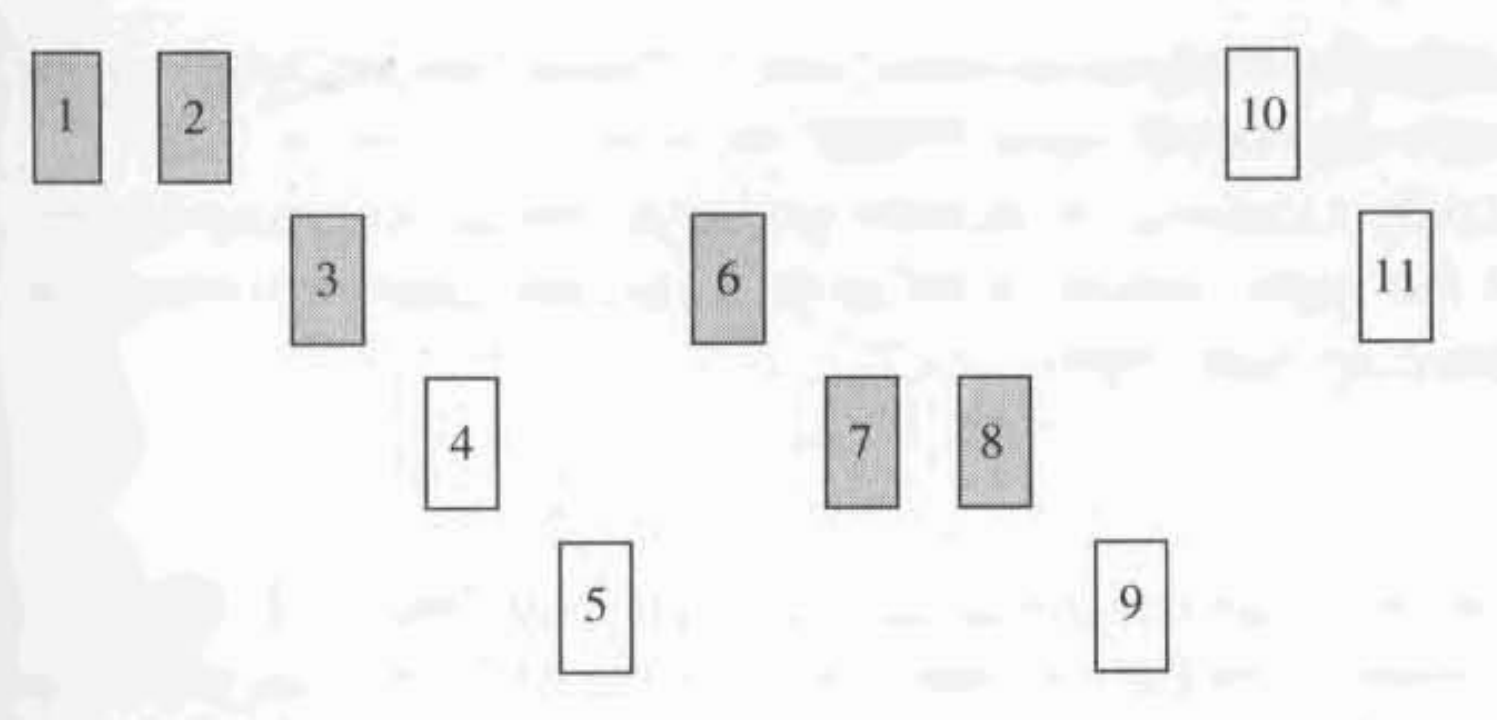
\includegraphics[width=0.4\textwidth]{Intervals_corresponding_to_the_conflict_graph}
    \caption{Intervals corresponding to the conflict graph. \cite{main}}
    \label{Intervals_corresponding_to_the_conflict_grap}
\end{figure}

In the next subtopic, we will discuss the method used to solve the binding problem for a given schedule and resource bound.


\subsection{ ILP model}

Binding problem for  circuit model whose specification include schedule and resource bound can be solved using ILP model \cite{main}. For the ILP model We use a set of binary decision variables with two indices, $ B=\{b_{ir};i=1,2,...,n_{pos};r=1,2,...,a\} $, and a set of binary decision constants with two indices, $ X=\{x_{il};i=1,2,...,n_{pos};l=1,2,...,\lambda+1\} $, where $ a\leq n_{ops} $ is an upper bound on the number of resources to be used, the binary variable,$ b_{ir} $ is 1 only when operation $ v_{i} $ is bound to resource r, i.e., $ \beta(v_{i})=(1,r) $ and the binary constant, $ x_{il} $ is 1 only when operation $ v_{i} $  starts in step 1 of the schedule, i.e., $ l = t{i} $ \cite{main}. 
Searching for a binding compatible with a given schedule (represented by $X$) and a resource bound $a$  is equivalent to searching for a set of values of B satisfying  the following constraints \cite{main}: 

\begin{equation}\label{a}
 \sum_{r=1}^{a} b_{ir} = 1, i=1,2,...,n_{ops} 
\end{equation}

\begin{equation}\label{b}
\sum_{i=1}^{n_{ops}} b_{ir}\sum_{m=l-d_{i}+1}^{l} x_{im} \leq 1, l=1,2,...,\lambda + 1, r=1,2,...,a 
\end{equation}

\begin{equation}\label{c}
b_{ir} \in \{0,1\}, 1 =1,2,...,n_{ops}, r=1,2,...,a
\end{equation}

 Based on our scheduled sequencing graph of ``Fig. \ref{scheduled_sequencing_graph}", the operations have two types and to make it simple we label multiplier with $1$ and ALU with $2$. So, a feasible binding satisfies the constraints \cite{main}: 

\begin{equation}\label{a}
 \sum_{r=1}^{a_{1}} b_{ir} = 1,\forall_{i} : \tau(v_{i})=1 
\end{equation}

\begin{equation}\label{b}
\sum_{i=:\tau(v_{i})=1}^{} b_{ir} x_{il} \leq 1, l=1,2,...,\lambda + 1, r=1,2,...,a_{1}
\end{equation}

\begin{equation}\label{c}
\sum_{r=1}^{a_{2}} b_{ir} = 1,\forall_{i} : \tau(v_{i})=2
\end{equation}

\begin{equation}\label{a}
 \sum_{i=:\tau(v_{i})=2}^{} b_{ir} x_{il} \leq 1, l=1,2,...,\lambda + 1, r=1,2,...,a_{2}
\end{equation}

The constants in the set X are all zero, except for $ x_{1,1},x_{1,1},x_{2,1},x_{3,2},x_{4,3},x_{5,4},x_{6,2},x_{7,3},x_{8,3},x_{9,4},x_{10,1},x_{11,2} $ which are 1. Then, an implementation with $ a_{1} =1$ multiplier would correspond to finding a solution to \cite{main} : 

\begin{equation}\label{b}
b_{i1} = 1, \forall_{i} \in \{1,2,3,6,7,8\}
\end{equation}

\begin{equation}\label{c}
\sum_{i\in \{1,2,3,6,7,8\}}^{} b_{i1} x_{il} \leq 1, l=1,2,...,5
\end{equation}


Such a solution does not exist, because the second constraint would imply $ b_{1,1}=b_{1,2} \leq 1 $, which contradicts the first one. An implementation with $ a_{1} =2$ multipliers would correspond to finding a solution to \cite{main}:


\begin{equation}\label{b}
 b_{i1}=b_{i2} = 1, \forall_{i} \in \{1,2,3,6,7,8\}
\end{equation}

\begin{equation}\label{c}
\sum_{i\in \{1,2,3,6,7,8\}}^{} b_{i1} x_{il} \leq 1, l=1,2,...,5
\end{equation}

\begin{equation}\label{c}
\sum_{i\in \{1,2,3,6,7,8\}}^{} b_{i2} x_{il} \leq 1, l=1,2,...,5
\end{equation}

which admits the solution $ b_{1,1}=1,b_{2,2}=1,b_{3,1}=1,b_{6,2}=1,b_{7,1}=1,b_{8,2}=1 $, all other elements of B with first subscript $ i \in \{I, 2,3.6,7,8\}$ being zero. The binding of the ALUs can be computed similarly. The list of binding is shown in ``Table \ref{tab1}" and can be illustrated using bound sequencing graph as shown in ``Fig. \ref{Scheduled_and_bound_sequencing}". The shaded area represent a resource and the operations within the shaded area are binded to the resource accordingly 


\begin{table}[htbp]
\caption{Binding result}
\begin{center}
\begin{tabular}{|c|c|c|c|}
\hline
$\beta(v_{1})$ & $(1,1)$  \\
$\beta(v_{2})$ &  $(1,2)$\\
$\beta(v_{3})$ &  $(1,1)$\\
$\beta(v_{4})$ &  $(2,1)$\\
$\beta(v_{5})$ &  $(2,1)$\\
$\beta(v_{6})$ &  $(1,2)$\\
$\beta(v_{7})$ &  $(1,1)$\\
$\beta(v_{8})$ &  $(1,2)$\\
$\beta(v_{9})$ &  $(2,2)$\\
$\beta(v_{10})$ &  $(2,1)$\\
$\beta(v_{11})$ &  $(2,1)$\\
\hline
\end{tabular}
\label{tab1}
\end{center}
\end{table}


\begin{figure}[h]
    \centering
    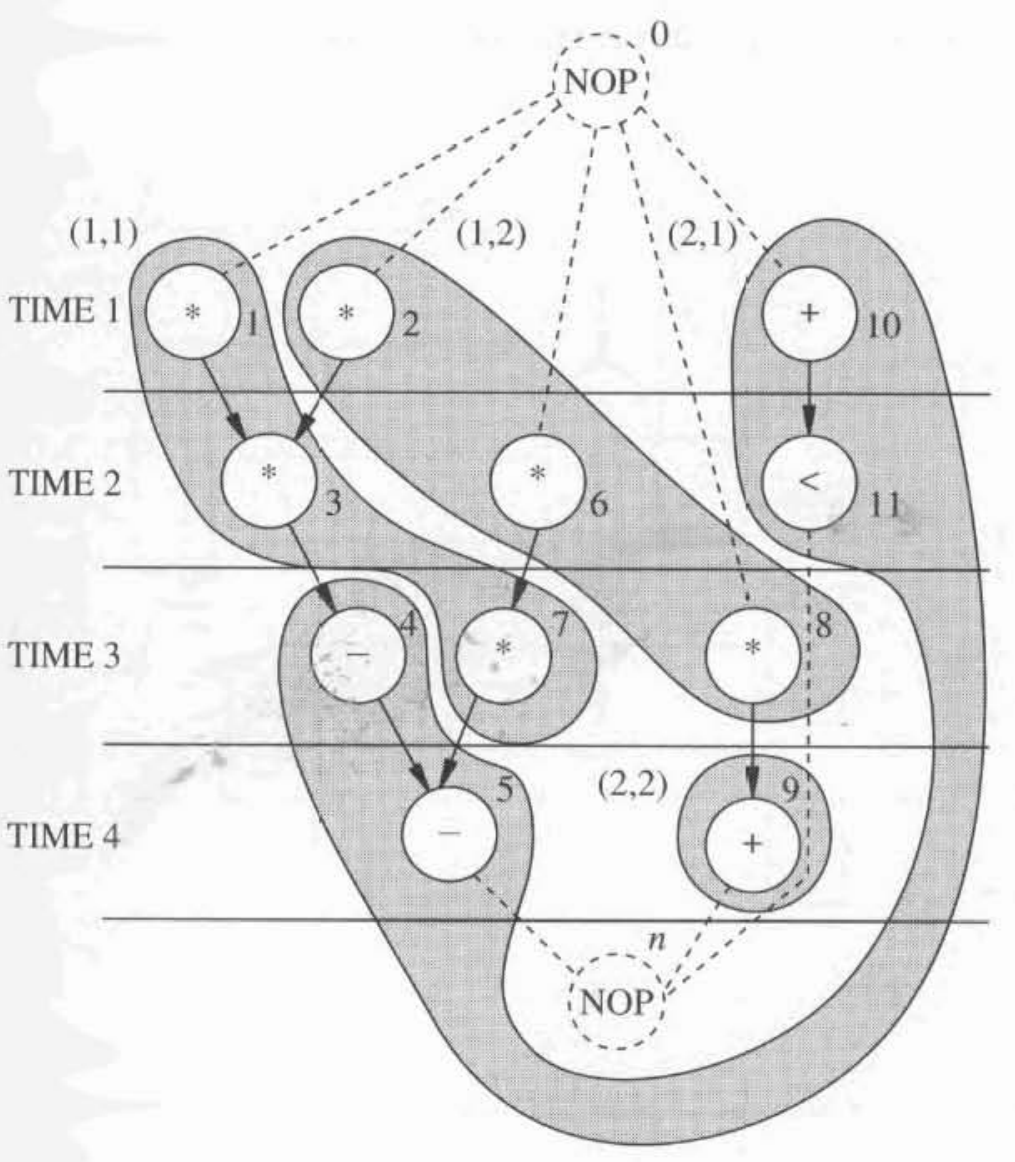
\includegraphics[width=0.4\textwidth]{Scheduled_and_bound_sequencing}
    \caption{Scheduled and bound sequencing. \cite{main}}
    \label{Scheduled_and_bound_sequencing}
\end{figure}



% sharing def
% binding def
% problem - The Spatial Domain: Binding 
% sharing and binding method 
% Non-Hierarchical Sequencing Graphs 
% Hierarchical Sequencing Graphs 
% Register Sharing 
% Multi-Port Memory Binding 
% Bus Sharing and Binding 
% UnconsIrGned Minimum-Area Binding* 
% Performance-ConsIrained and Performance-Directed Binding*


\section{Optimization}
% area and performance estimation
% design space
% optimization : 3 trade-off


The evaluation of a circuit is through its used area and performance. This aspect can be only optimized during the architectural synthesis. So it is important to have the ability to estimate the area used and resulted performance. This then used to make further optimization until the optimum circuit can be produce. The area and performance estimation and optimization during high level synthesis can be done during sharing and binding process. This is due to the fact that a binding provide the information about the area of a circuit and schedule provide the latency with given cycle-time. In this section, we will go through the step in estimating area and performance of a circuit. Then we will go further with the optimization strategies.



\subsection{Area and performance estimation}

In general circuit, the total area of a circuit is the sum of area of resource, steering logic, register, control unit and wiring area. The number of those component used in a circuit is depends on binding as well as schedule. Reducing the number of used resource linearly does not mean that area is reduced linearly. As we discussed in pervious section, resource sharing is applied to reduce used area and reducing the number of resource also cause the increasing number of steering logic, register and control unit. That means the number of every single component affect the used area.

Circuit performance can be evaluated through circuit schedule. As we discussed before in pervious section, schedule sequencing graph provide us the value of latency, $\lambda$ , propagation delay of an operation and cycle-time. Since the value of latency with defined cycle-time affected by binding, that give us information about maximum number of operation with the same type can run concurrently, we can also estimate the performance through binding. Binding explicitly describe the type and number of component being used. That means every single component affect the performance because the number of resource affect the total of propagation delay and latency.

So it is important to know how the number of every single component such as resource, steering logic, wiring and control unit affect the area and performance. The list below explain how The components affect the area and performance \cite{main}.

\begin{itemize}
    \item Resource : A resource affect the area and performance through its size and its propagation delays of combinational logic.
    \item Steering logic : Steering logic affect the propagation delay of a resource. The effected area can be estimated depend on the number of input and out put of a multiplexer used as we discuss in pervious section. 
    \item wiring : Wiring contribute to overall area and delay. Estimating the wiring area and length requires the knowledge of the structure. The delay cause by wiring can be estimated through its length.
    \item Control unit : Control unit contribute to overall area and delay. The area of control unit can be estimate based on latency because the word length used to accommodate all control step can be estimated.
\end{itemize}

Next, which is the last step in our synthesizing process will be discussed, which is optimization strategies.

\subsection{Optimization strategies}

In this subsection, we will discuss circuit optimization. Optimization process involve scheduling and binding in order to optimize the area, latency and cycle-time because of the aim of architectural optimization is to find a scheduled sequencing graph with a complete resource binding that met all the given constraints \cite{main}. An optimum circuit can be built if the circuit is not influenced only by one aspect, e.g. area, but fairly influenced by all aspect. As explained in pervious section, particularly in compatibility graph subsection, we can see that reducing number of resource cause more operation need to share some resource, thus the operation cannot run concurrently, and the latency need to be increased. On the other hand, increasing the number of resource could reduce the latency but increase the total area of a circuit. Reducing the cycle time could cause an operation to take two cycles to complete. All the possibilities can be structure in design evaluation space. To have an optimum circuit, we need to find a point where all aspects are fairly dominate the circuit. This point is called Pareto point \cite{main}.


To have this point, a designer should traverse the design evaluation space. Architectural exploration is often done by exploring the (area/latency) trade-off for different values of the cycle-time \cite{main}. Another approach is through search for the (cycle-time/latency) tradeoff for some binding or the (area/cycle-time) trade-off for some schedules.

Next we will go through for each design evaluation space.

\subsection{(area/latency) trade-off}

In (area/latency) trade-off design evaluation space, the value of cycle time is fixed. The extreme point of each aspect, area and latency, can be found by finding the minimum value of latency and resource accordingly. The design evaluation space can be explored by reducing one parameter as a function of the other. 

Based on our circuit model as in ``Fig. \ref{scheduled_sequencing_graph}", we make assumption as below : 
\begin{itemize}
    \item Area constraint is 20 units.
    \item Latency less than 8 cycles.
    \item ALU propagation delay is 25 ns.
    \item Multiplier propagation delay is 35 ns.
\end{itemize}

Since the cycle time should be fixed, if we set the cycle-time to 40ns, every operation will take one cycle time, but if we set it to 30ns, multiplier will take two cycles to complete. Now we fix our cycle time to 40ns.

If we took only one multiplier, the resulting latency is 13, and it will break the constraint. if we choose two multiplier and one adder, the resulting latency and area is 8 cycles and 12 unit. The exploration can be continued by trying all the possibilities as shown in ``Fig. \ref{Design_evaluation_space_area_latency_Trade_off_points_for_two_values_of_the_cycle-rime}".

\begin{figure}[ht]
    \centering
    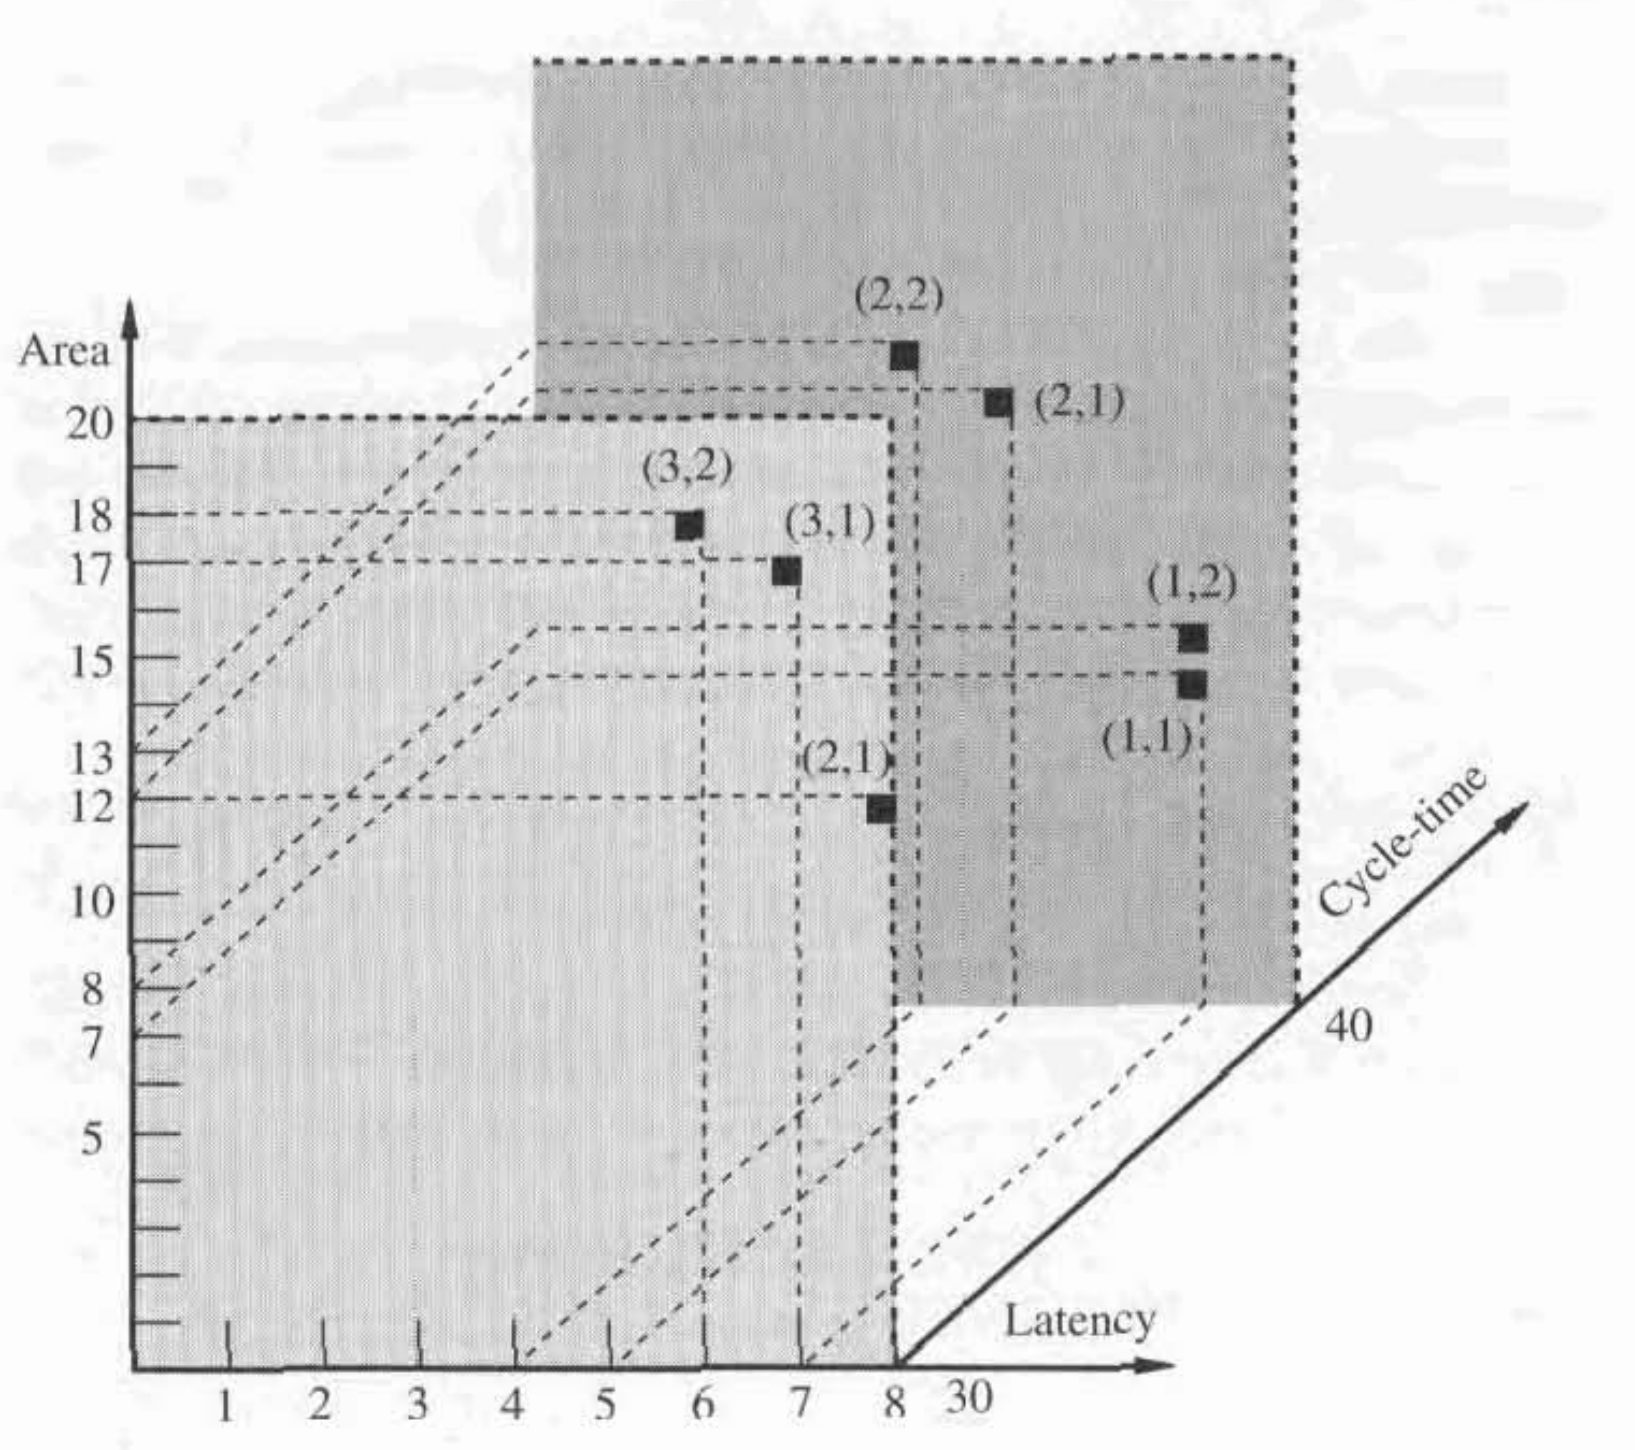
\includegraphics[width=0.4\textwidth]{Design_evaluation_space_area_latency_Trade_off_points_for_two_values_of_the_cycle-rime}
    \caption{Design evaluation space: area/latency trade off points for two values of the cycle time. \cite{main}}
    \label{Design_evaluation_space_area_latency_Trade_off_points_for_two_values_of_the_cycle-rime}
\end{figure}


\subsection{(cycle-time/latency) trade-off}

By fixing the value of total area, we could try to draw a possible point by changing the value of number of component and see how the value of cycle-time and latency affect each other as shown in ``Fig.\ref{Design_evaluation_space_some_cycle_timenatency_trade-off_points_for_two_bindings}". From our discussion in the pervious section, the method that used weighted compatibility graph could be helpful.  

\begin{figure}[ht]
    \centering
    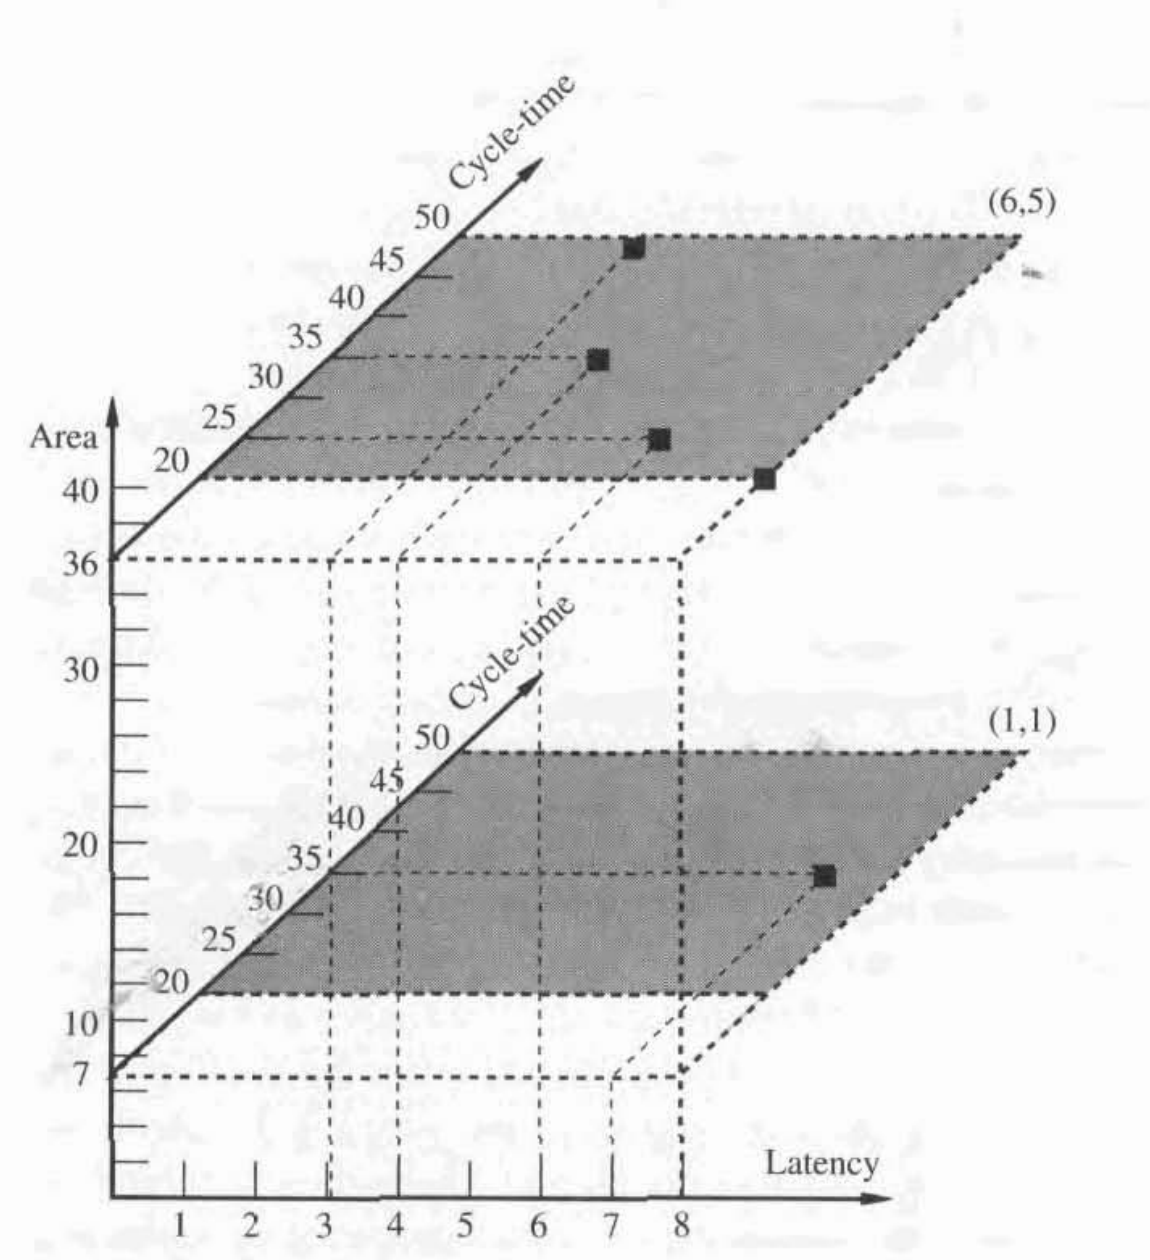
\includegraphics[width=0.4\textwidth]{Design_evaluation_space_some_cycle_timenatency_trade-off_points_for_two_bindings}
    \caption{Design evaluation space: cycle-time/latency trade off points for two values of the area. \cite{main}}
    \label{Design_evaluation_space_some_cycle_timenatency_trade-off_points_for_two_bindings}
\end{figure}


\subsection{(area/cycle-time) trade-off}

By fixing the value of latency, we could try to draw a possible point by changing the value of number of component and see how the value of cycle-time and area affect each other as shown in ``Fig.\ref{Desisn_evilluatinn_apace_some_cycle_timellarcncytmde_of_points_far_wo}" by applying possible methods from pervious section.

\begin{figure}[ht]
    \centering
    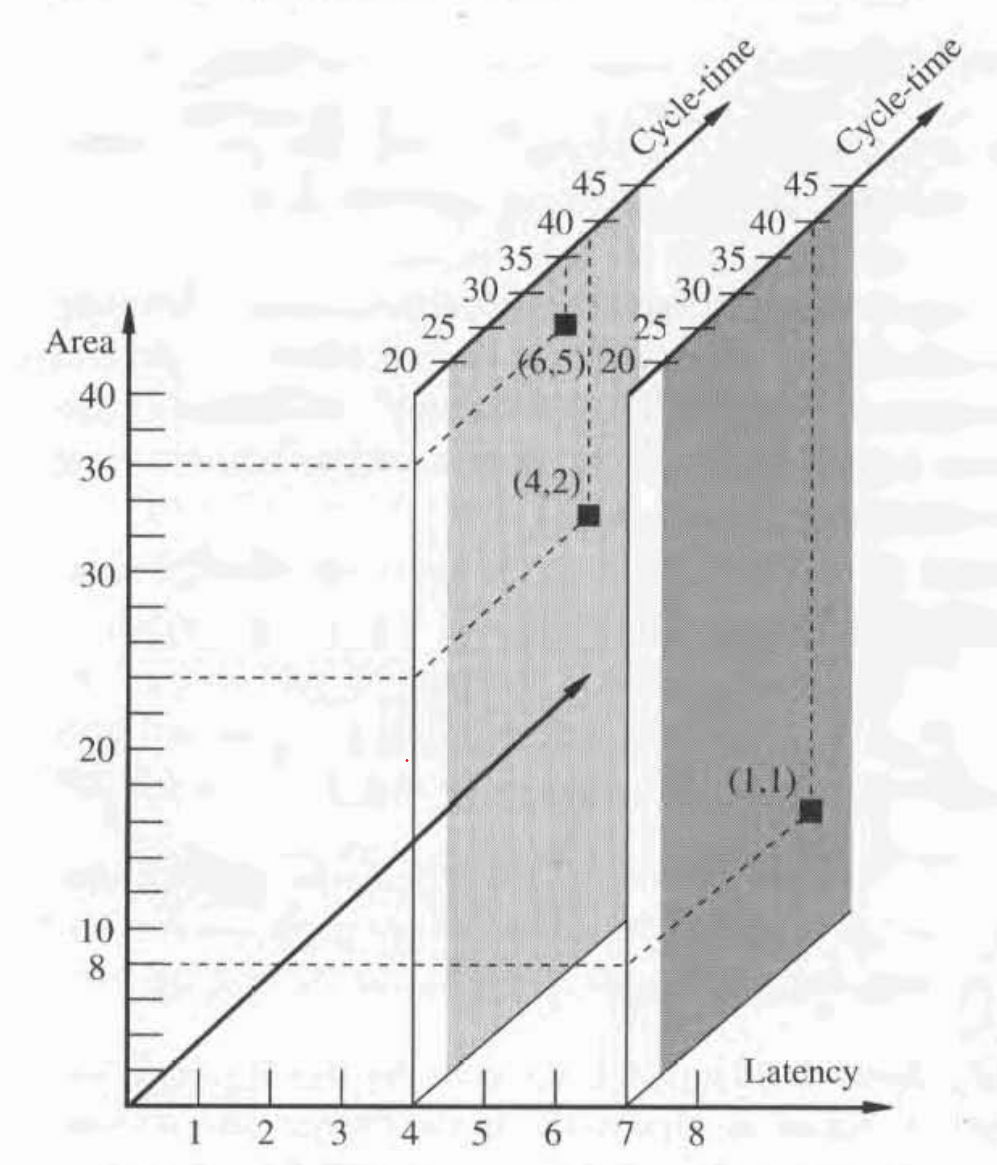
\includegraphics[width=0.4\textwidth]{Desisn_evilluatinn_apace_some_cycle_timellarcncytmde_of_points_far_wo}
    \caption{Design evaluation space: area/cycle-time trade off points for two values of the latency. \cite{main}}
    \label{Desisn_evilluatinn_apace_some_cycle_timellarcncytmde_of_points_far_wo}
\end{figure}



% area and performance estimation
% design space
% optimization : 3 trade-off

\section{Conclusion}

%important of binding.   -- in producing optimum circuit.
%important of all knowledge.
%importance of optimization

As a conclusion, since the optimization of a circuit can only be done during  high level synthesis, it is important to have concrete understanding how sharing and binding affect the area and performance of a circuit and the methods to implement them. The design evaluation space also needs to be comprehended to allow a designer to find the Pareto point in order to produce an optimum circuit.  The exploration of design evaluation space can be improved not only through learned theory, but also experience.


\section*{Acknowledgment}
I would like to express my very great appreciation to Dr Achim Rettberg for his valuable and constructive suggestions during the planning and development of this research work. His willingness to give his time so generously has been very much appreciated.

\begin{thebibliography}{00}
\bibitem{main} G. D. Micheli, Synthesis and optimization of digital circuits. New York: McGraw-Hill, 1994.
\bibitem{b2} Shilpa, K. and Lakshminarayana, C and Singh, Manoj. (2019). Optimal Resource Allocation and Binding in High-Level Synthesis Using Nature-Inspired Computation. 10.1007/978-981-13-5802-9-95.  
\end{thebibliography}


\end{document}
